% !TEX ROOT = ../ersti.tex
\section{Verkehrsmittel in Heidelberg}
\label{verkehrsmittel}

\begin{figure*}[b]
    \centering
    \begin{subfigure}{.24\textwidth}
	
\includegraphics[height=5cm]{bilder/vacuum_1.png}
    \end{subfigure}
    \begin{subfigure}{.24\textwidth}
	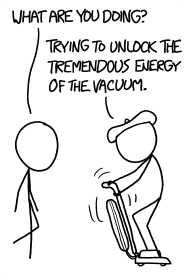
\includegraphics[height=5cm]{bilder/vacuum_2.png}
    \end{subfigure}
    \begin{subfigure}{.24\textwidth}
	
\includegraphics[height=5cm]{bilder/vacuum_3.png}
    \end{subfigure}
    \begin{subfigure}{.24\textwidth}
	
\includegraphics[height=5cm]{bilder/vacuum_4.png}
    \end{subfigure}
\end{figure*}


Besorg' dir ein Fahrrad! Es ist das schnellste, zuverlässigste und auch günstigste\footnote{Wenn du dich an die StVo hälst -- oder dich nicht erwischen lässt.} Verkehrsmittel in Heidelberg. Für fast alle wichtigen Routen gibt es Radstreifen oder ausgeschilderte Wege über Seitenstraßen, sodass man vom Berufsverkehr weitgehend verschont bleibt. Selbst für die Distanzen auf dem Campus kann sich eine Anschaffung lohnen: vom Hörsaal über die \gls{UB} zur Mensa läuft man gerne 15 Minuten. Auch abends, wenn die Bahnen nur noch halbstündlich oder gar nicht mehr fahren, ist das Fahrrad oft die bessere Alternative. Und falls es mal kaputt geht, schaust du einfach im \emph{URRmEL}\footnote{Öffnungszeiten: Di \& Do von 16 - 20 Uhr} vorbei, der Uni-eigenen Fahrradwerkstatt. Da musst du dein Fahrrad zwar selber reparieren, dafür sind aber immer Leute da, die dir sagen wie das geht und dir auch mal helfen. An Werkzeugen und Ersatzteilen herrscht auch kein Mangel.

\label{nextbike}
Wenn du am Anfang kein Fahrrad hast oder dein Fahrrad verloren gegangen ist, gibt es seit dem Sommersemester 2018 die Möglichkeit für 30 Minuten ein Fahrrad kostenlos von VRNnextbike\footnote{Finanziert wird dies durch einen Solidarbeitrag ähnlich zum Semesterticket in Höhe von \EUR{2,40}.} zu leihen. Nach den kostenlosen 30 Minuten kostet jede halbe Stunde 50 Cent. Wird das Fahrrad vorher abgegeben, so wird für die Benutzerin für 15 Minuten die kostenlose Mietoption "gesperrt". Die Rückgabe und Ausleihe ist an diversen Standorten in Heidelberg und Umgebung über Hotline, App oder an der Station selbst möglich. Auch im Urlaub in einigen Städten Deutschlands kann der kostenlose Grundtarif verwendet werden\footnote{Mehr Informationen über Nextbike findest du beim StuRa unter \url{https://www.stura.uni-heidelberg.de/referate/verkehr/vrnextbike.html}}.

Wenn du doch mal Bus oder Bahn nutzen willst, brauchst du nicht gleich ein Ticket kaufen: ab 19 Uhr, am ganzen Wochenende und an gesetzlichen Feiertagen gilt dein Studiausweis als Fahrkarte im Stadtgebiet\footnote{Wabe 125, das ist Heidelberg inkl. aller Stadtteile} und angrenzenden Gemeinden\footnote{Waben 105, 135, 145 bzw. Eppelheim, Dossenheim, Schriesheim, Leimen, Sandhausen}. Bezahlt hast du dafür bereits mit einem Solidarbeitrag innerhalb der \EUR{\beitragssumme}, die du Anfang des Semesters überwiesen hast.

Sollte dir das nicht reichen, weil du z.B. in die Heimat pendeln willst, gibt es noch das Semesterticket. Da es sich in den letzten Jahren stark verteuert hat (um 146\%) ist es jedoch nicht mehr uneingeschränkt zu empfehlen. Das Ticket gilt im ganzen VRN Gebiet ohne Westpfalz sowie einigen Übergangsgebieten und kostet \EUR{\semesterticket}. Wie man dem Wabenplan\footnote{\url{http://www.vrn.de/vrn/tickets/tarifsystem/wabenplan}} des \glspl{VRN} entnehmen kann, kommt man dann zwar gut von Ost nach West, aber in Nord-Süd Richtung ist nach einigen Kilometern Schluss. Leider zeigte der \gls{VRN} in Verhandlungen auch kein Interesse, das Ticket durch z.B. Direktverbindungen in die umliegenden Großstädte attraktiver zu machen.

%In jedem Fall lohnt ein Vergleich der Ticketkosten mit denen für eine BahnCard. Letztere ist deutlich flexibler, was das Ziel anbelangt und je nach dem wie oft man vorhat zu pendeln sogar günstiger.

Bleibt noch das Auto. Sofern du nicht unglaublich viel Geld, Zeit und Nerven hast um die Parkplatzsuche und den Berufsverkehr zu bewältigen, kann man vom Auto nur abraten. Zum Pendeln in die Heimat am Wochenende ist es sicher noch zu gebrauchen, sofern du hier leicht Zugang zu einem Parkplatz hast. Wer täglich pendeln will oder muss, parkt jedoch besser weit außerhalb und legt den Rest mit \gls{OPNV} oder Fahrrad zurück.


\begin{figure*}[!b]
\centering{
    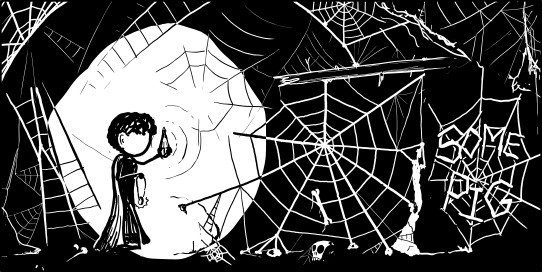
\includegraphics[width=\textwidth]{bilder/cirith_ungol.png}
}
\end{figure*}

